\documentclass[tikz]{standalone}

\begin{document}
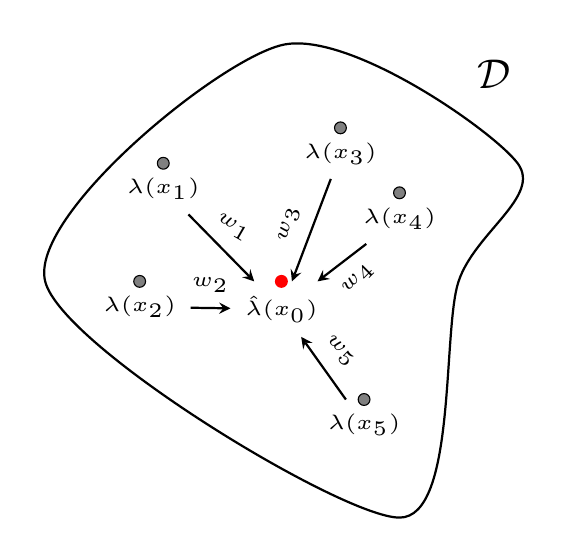
\begin{tikzpicture}[scale=1.5,transform shape]
\draw [thick,black] plot [smooth cycle] coordinates {(0,0) (2,2) (4,1) (3.5,0) (3,-2)};

\draw[fill=gray] (1,1) circle [radius=0.05];
\node [below] at (1,1) (A) {\tiny $\lambda(x_1)$};
\draw[fill=gray] (0.8,0) circle [radius=0.05];
\node [below] at (0.8,0) (B) {\tiny $\lambda(x_2)$};
\draw[fill=gray] (2.5,1.3) circle [radius=0.05];
\node [below] at (2.5,1.3) (C){\tiny $\lambda(x_3)$};
\draw[fill=gray] (3,0.75) circle [radius=0.05];
\node [below] at (3,0.75) (D) {\tiny $\lambda(x_4)$};
\draw[fill=gray] (2.7,-1) circle [radius=0.05];
\node [below] at (2.7,-1) (E) {\tiny $\lambda(x_5)$};

\draw[fill=magenta, red] (2,0) circle [radius=0.05];
\node [below] at (2,0) (F) {\tiny $\hat{\lambda}(x_0)$};

\draw [thick,-stealth] (A) -- (F) node[midway,above,rotate=-30] {\tiny $w_1$};
\draw [thick,-stealth] (B) -- (F) node[midway,above] {\tiny $w_2$};
\draw [thick,-stealth] (C) -- (F) node[midway, above, rotate=75] {\tiny $w_3$};
\draw [thick,-stealth] (D) -- (F) node[midway, below, rotate=45] {\tiny $w_4$};
\draw [thick,-stealth] (E) -- (F) node[midway, above, rotate=-45] {\tiny $w_5$};

\node [below] at (3.8,2) {$\mathcal{D}$};
\end{tikzpicture}
\end{document}
